\chapter{Background}
\label{chap:background}

\todo{Ákos dipterv}


\section{Mathematical logic}

\subsection{Zeroth order logic}
SAT
\subsection{First order logic}
SMT

\section{Formal verification}
\todo{Importance, etc.}
\subsection{Timed automata}
\todo{Modeling formalisms, timed systems, etc.}

\subsubsection{Basic Definitions}
In order to properly define timed automata, first the idea of \emph{clock variables} must be explained. In case of systems with discrete variables, the values of the variables always remain the same betrween two modifications. However, this is not the case for clock variables (clocks, for short). Even when a system stays in one state, the value of clocks are continuously and steadily increasing. Naturally, their values can be modified, but the only allowed operation on clock variables is \emph{reset}. Reseting a clock means assigning its value to a specific integer (often, that integer can only be 0). It's an instantaneous operation, after which the value of the clock will continue to increase.

Hereinafter follows some basic definitions that are closely related to clock variables and timed automata. 

\begin{dfn}
	A \emph{valuation} $v(\mathcal{C})$ assigns a non-negative real value
	to each clock variable $c \in \mathcal{C}$, where $\mathcal{C}$ denotes the set of clock
	variables.
\end{dfn}

In other words a valuation defines the values of the clocks at a given moment of time. The term \emph{valuation} can also be used for discrete variables.

\begin{dfn}
	A \emph{clock constraint} is a conjunctive formula of atomic
	constraints of the form $x \sim n$ or $x - y \sim n$ (\emph{difference
		constraint}), where $x,y \in \mathcal{C}$ are clock variables, $\sim \in
	\{\leq,<,=,>,\geq\}$ and \hbox{$n \in \mathbb{N}$}. $\mathcal{B}(\mathcal{C})$ represents the set of clock
	constraints.
\end{dfn}

In other words a clock constraint defines upper and lower bounds on the values of clocks (or differences of clocks, in case of difference constraints). Bounds are always integer numbers. Clock constraints are used in guards and invariants of timed automata to control the behaviour by only allowing certain operations if the current valuation satisfies the consraints. 

A \emph{timed automaton} extends a finite automaton with clock variables. It can be defined as follows.

\begin{dfn}
A \emph{timed automaton} $\mathcal{A}$ is a tuple $\langle L, l_0,
E, I\rangle$ where
\begin{itemize}
	\item $L$ is the set of locations,
	\item $l_0 \in L$ is the initial location,
	\item $E \subseteq L \times \mathcal{B}(\mathcal{C}) \times 2^\mathcal{C} \times L$ is the set of edges and
	\item $I: L \to \mathcal{B}(\mathcal{C})$ assigns invariants to locations.  Invariants can be used to ensure the progress of time in the model. \cite{bengtsson2004timed}
\end{itemize}
\end{dfn}

Graphically a timed automaton can be represented as a labeled graph where the vertices are the locations labelled with their corresponding invariants, and the edges are the automaton's edges, that are defined by the source location, the guard (represented by a clock constraint), the set of clocks to reset, and the target location.

\todo{példa}

A state of $\mathcal{A}$ is a pair $\langle l,v \rangle$ where $l \in L$ is a
location and $v$ is the current valuation satisfying $I(l)$. In the initial
state $\langle l_0,v_0 \rangle$ $v_0$ assigns 0 to each clock variable.

Two kinds of operations are defined. The state $\langle l,v \rangle$ has a
\emph{discrete transition} to $\langle l',v' \rangle$  if there is an
edge $e(l,g,r,l') \in E$ in the automaton such that 
\begin{itemize}
	\item $v$ satisfies $g$, 
	\item $v'$ assigns 0 to any $c \in r$ and assigns $v(c)$ to any $c \not\in r$, and
	\item $v'$ satisfies $I(l')$. 
\end{itemize}
The state $\langle l,v \rangle$ has a \emph{time transition} (or delay, for short) to $\langle l,v' \rangle$ if
\begin{itemize}
	\item $v'$ assigns $v(c)+d$ for some non-negative $d$ to each $c \in \mathcal{C}$ and
	\item $v'$ satisfies $I(l)$. 
\end{itemize}


There are many variations of timed automata (e.g. this definition only allows to reset clocks to 0, however, resets to greater integers will appear later in this paper). Most of them such as network automata, synchronization, and urgent locations can be easily transformed into conventional timed automata, but this is not always the case. The idea to allow discrete variables as well as clock variables arises simply. Bool, integer, rational, or even self-described typed variables prove useful, but may result in a formalism with bigger expressive power that that of the conventional timed automaton. This becomes important when one wants to analyze a system.


\subsection{Reachability}

\todo{Importance, basic algorithms (statespace exploration, SAT based solution, bounded stuff + examples), TA reachability + examples}

\subsubsection{Timed automaton reachability} \label{sec:tareach}

\todo{complexity, complextity w/ disc vars, encoding disc vars in locations, etc}

\subsection{CEGAR}
\subsubsection{Abstraction}
Idea, usefulness, Times automata - zones, variables, activity, etc.
\subsubsection{CEGAR-loop}
Idea, Cegar-loop, basic cegar ideas (variable-based, statespace refinement, etc.)
%This chapter defines the important aspects of timed automata and briefly explains the reachability algorithm presented in \cite{bengtsson2004timed} and demonstrates it on some examples (based on examples, also from \cite{bengtsson2004timed}). CEGAR is also explained at a high level.


%\section{Timed Automata}

%\subsection{Reachability Analysis} \label{sec:reach}  
%
%A \emph{zone} is a set of nonnegative clock valuations satisfying a set of clock constraints.
%The set of all valuations reachable from a zone $z$ by time transitions is denoted by $z^\uparrow$.
%
%A \emph{zone graph} is a finite graph consisting of $\langle l,z \rangle$ pairs as nodes, where $l \in L$ refers to some
%location of a timed automaton and $z$ is a zone. Therefore, a node denotes a set
%of states. Edges between nodes denote transitions. 
%
%The construction of the graph starts with the initial node  $\langle l_0,z_0 \rangle$,
%where $l_0$ is the initial location and $z_0$ contains the valuations reachable in the initial location by time transitions. 
%Next, for each outgoing edge $e$ of the initial location (in the automaton) a new node  $\langle l,z \rangle$ is created (in the zone graph) with an edge
%$\langle l_0,z_0 \rangle \to \langle l,z \rangle$, where $\langle l,z \rangle$ contains the states to which the states in $\langle l_0,z_0 \rangle$ have a discrete transition through $e$. Afterwards $z$ is replaced by $z^\uparrow$.  The procedure is repeated on every newly introduced node of the zone graph. If the states defined by a newly introduced node $\langle l,z \rangle$ are all contained in an already existing node $\langle l,z' \rangle$, $\langle l,z \rangle$ can be removed, and the incoming edge should be redirected to $\langle l,z' \rangle$.
%
%\begin{figure} [h]
%	\centering
%	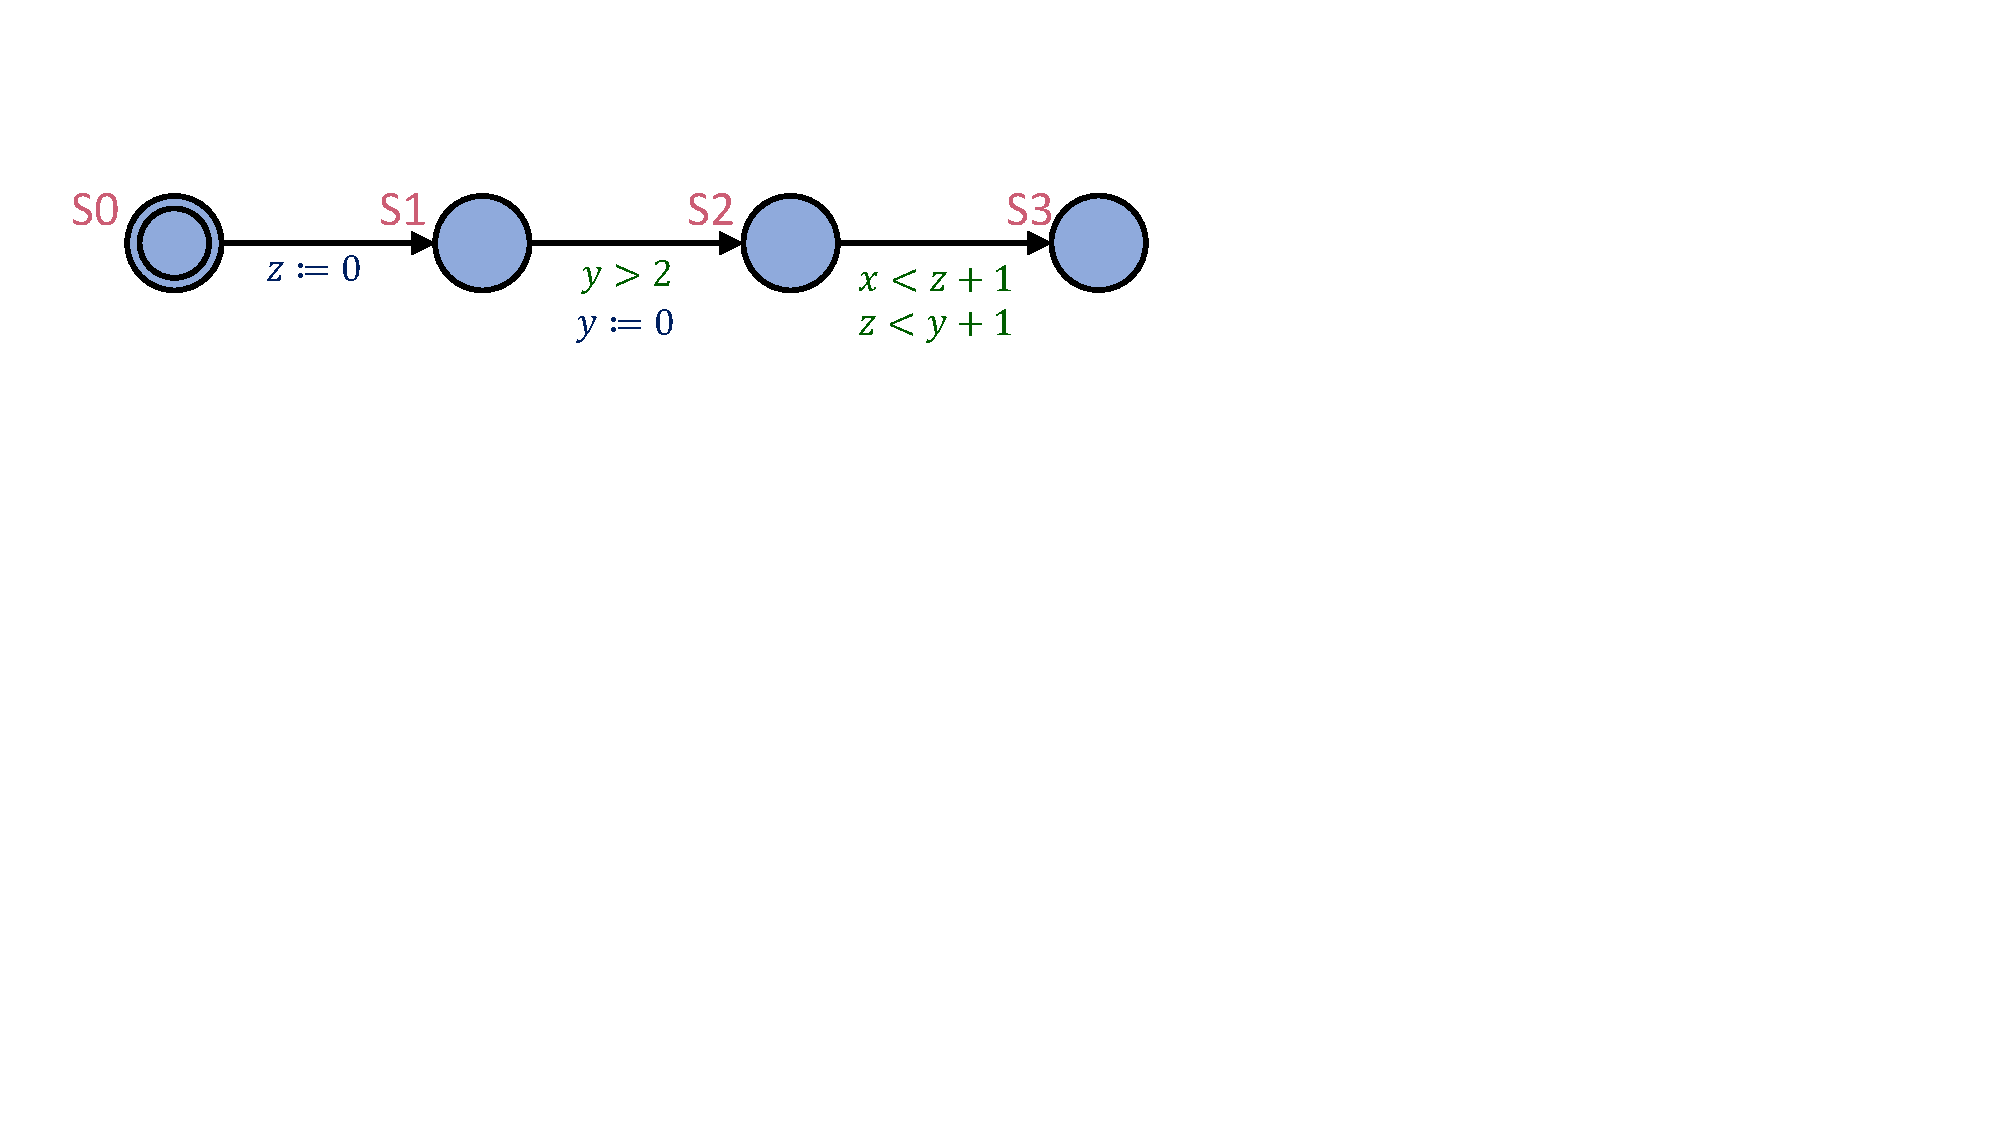
\includegraphics[width=.7\textwidth]{include/figures/splitexample_aut}
%	\caption{Timed automaton example}
%	\label{fig:splitex}
%\end{figure}  
%
%
%\begin{example}
%	
%
%
%For ease of understanding the algorithm is demonstrated on the automaton in Figure \ref{fig:splitex}. The inital state is  $\langle S0, z_0 \rangle$ where $z_0$ is a zone containing only the initial valuation $v_0 \equiv 0$. The initial node is  $\langle start, z_0^\uparrow  \rangle$, where $z_0^\uparrow$ contains all states reachable form the initial state by delay. Since as time passes, the values of the three clocks will be incremented by the same value, $x$, $y$ and $z$ has the same value in each valuation contained by $z_0^\uparrow$. Since there is no invariant in location $S0$ the clocks can take any positive value. Because of this $z_0$ can be defined by the constraint $x=y=z$ (that is, $x-y = 0 \wedge y-z=0 $), and the initial node can be defined as $\langle S0; x=y=z  \rangle$.
%
%There is only one outgoing transition from the initial location and that resets $z$, resulting in the zone defined by $x=y \wedge z=0$, which transforms into $z \leq x=y$ when delay is applied. This means the next node of the graph can be defined as $\langle S1, z \leq x=y \rangle$. There is only one outgoing transition from the location $S1$ and it has guard $y>2$. This means the transition is only enabled in the subzone $z \leq x=y>2$ (that is $z \leq x \wedge x=y \wedge y>2$). Th transition resets $y$ resulting in the zone $y=0 \wedge z \leq x > 2$. Delay can be applied and the next node of the graph turns out to be $\langle S2, z \leq x \wedge y \leq z \wedge x-y>2 \rangle$.
%
%There outgoing transition from location $S2$ has a guard $x<z+1 \wedge z<y+1$ from which we can determine $x<y+2$ contradicting the atomic constraint $x-y>2$ in the reachable zone of location $S2$. Thus the transition is never enabled, and location $S3$ is unreachable.  
%
%%The invariant $x \leq 10$ of location $loop$ is satisfied by $z_0$, but we have to consider it when calculating the valuations reachable by delay - only the states satisfying $x \leq 10$ of $z_0^\uparrow$ are reachable. The node of the graph can be defined as $\langle loop, x=y \wedge x<10 \rangle$.
%
%%Since there is no state in $\langle loop, x=y \wedge x \leq 10 \rangle$ where $y \geq 20$ holds, the last transition will never be enabled and the zone graph is finished.
%The resulting zone graph is the following.
%
%	\[\langle S0; x=y=z  \rangle \rightarrow \langle S1, z \leq x=y \rangle \rightarrow \langle S2, z \leq x \wedge y \leq z \wedge x-y>2 \rangle \]
%
%\end{example}
%
%\begin{figure} [b]
%	\centering
%	\begin{minipage}[c] {0.25\linewidth}%
%		%		\vspace*{1pt}%
%		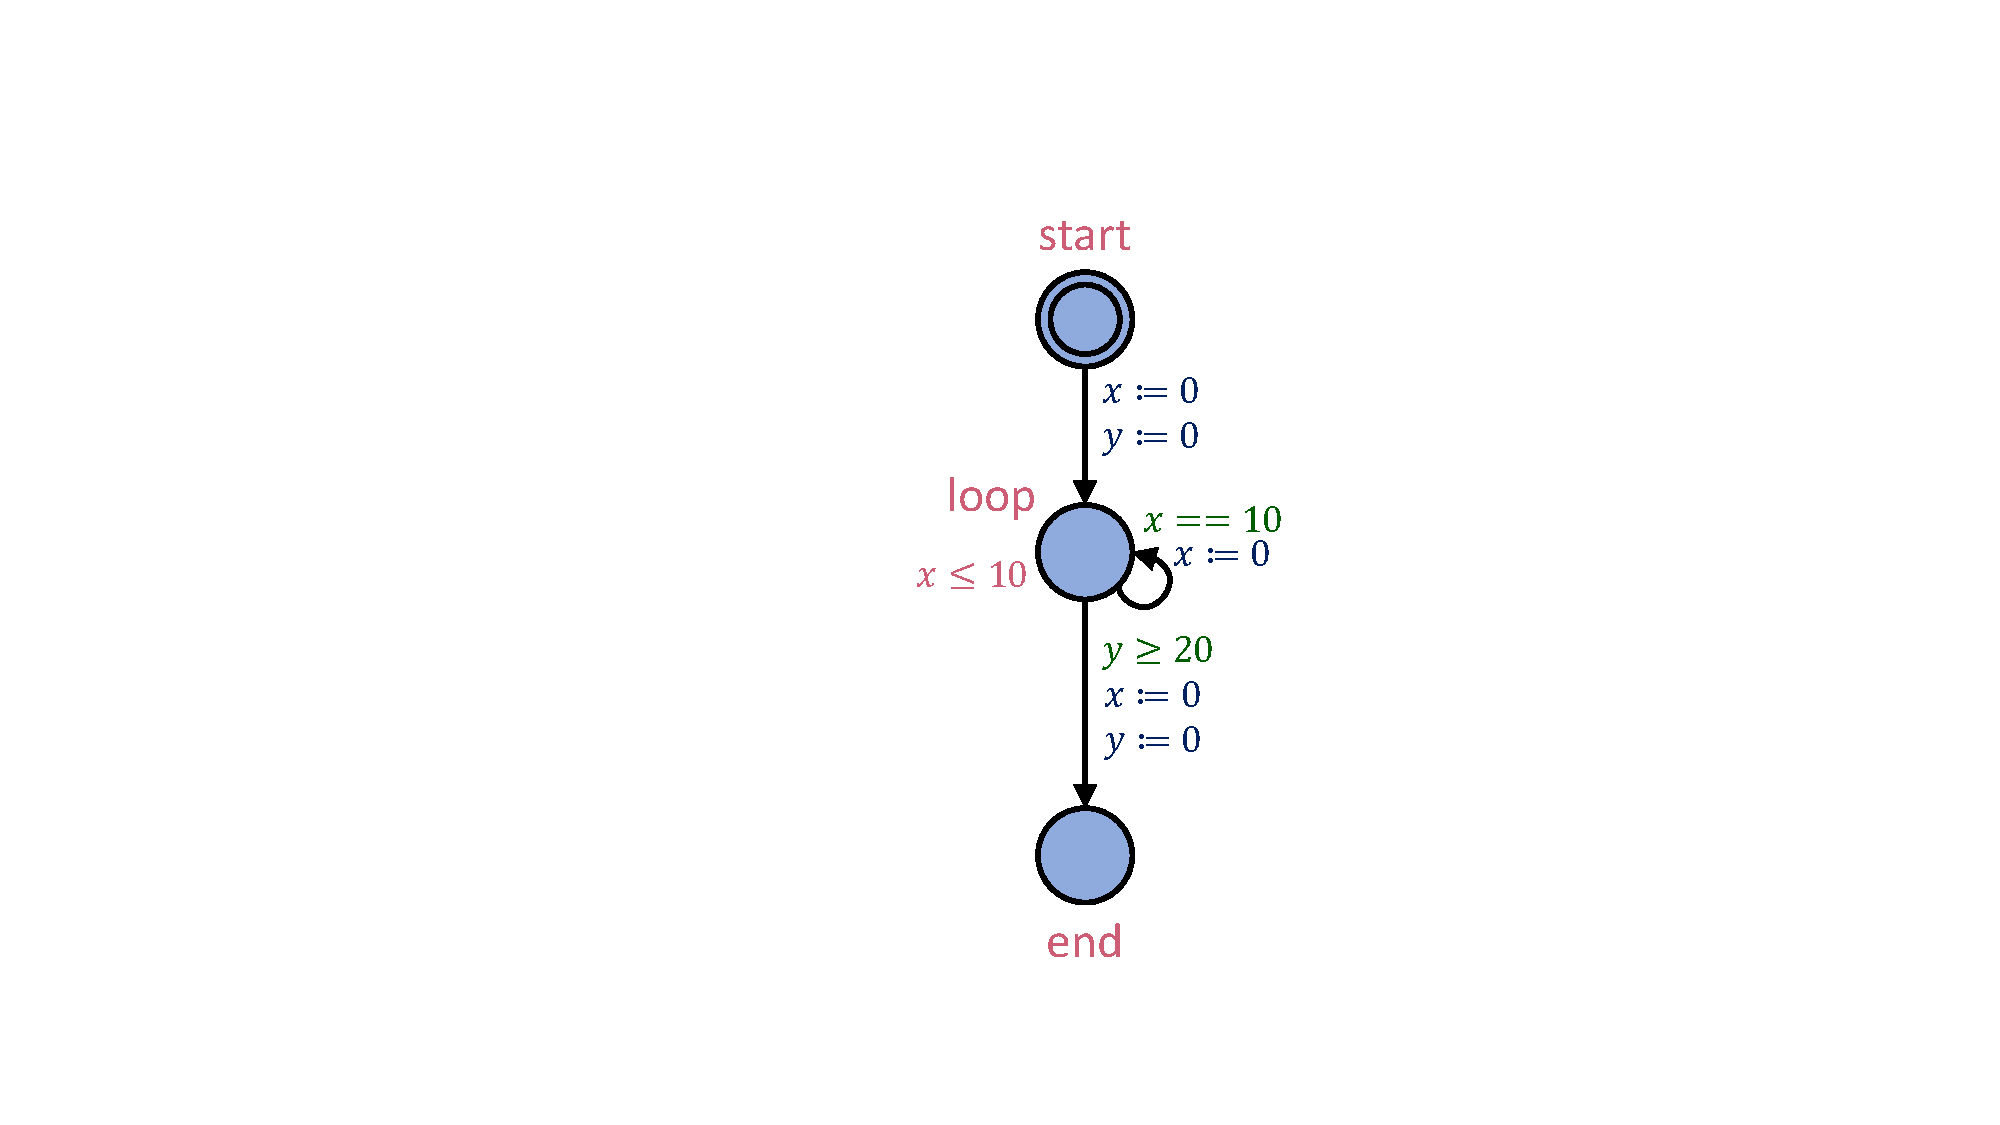
\includegraphics [width=\textwidth]{include/figures/loop_example_original}%
%		%\caption{Example of a timed automaton}
%	\end{minipage}%
%	%	%
%	\begin{minipage}[c] {0.7\linewidth}%
%		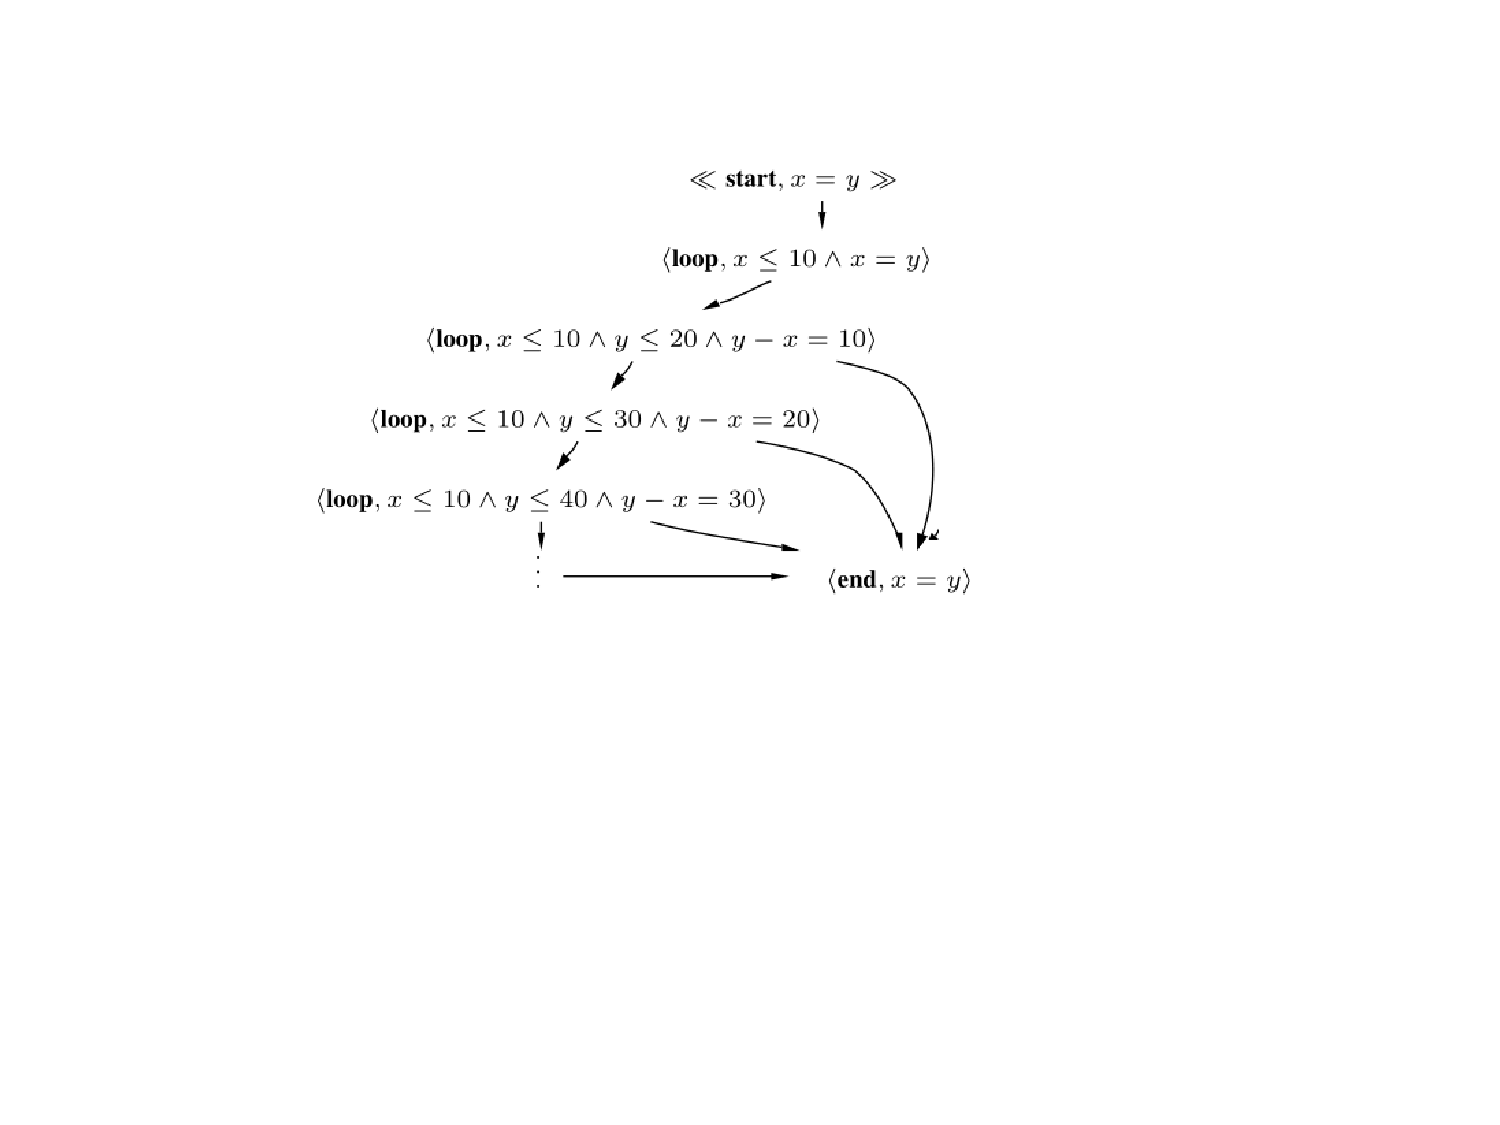
\includegraphics [width=\textwidth] {include/figures/loop_original_zonegraph}%TODO: ezt majd még vektorosítani
%		%		\vspace*{4pt}%
%		%		\caption{Timed automaton}
%	\end{minipage}
%	\caption{Timed automaton with infinite zone graph}
%	\label{fig:loopinfinite}
%\end{figure} 
%
%Unfortunately, it is possible that the graph described by the previous algorithm becomes infinite. Consider for example the automaton from \cite{bengtsson2004timed} in Figure \ref{fig:loopinfinite}.
%
%\begin{example}
%Constructing the zone graph of this automaton starts similarly, with the node $\langle start, x=y \rangle$. After that both $x$ and $y$ are reset resulting in the zone defined by $x=y=0$. Location $loop$ has an invariant $x \leq 10$ that limits the applicable delay to 10, resulting in $\langle loop, x=y \leq 10 \rangle$, where only the loop-transition is enabled.
%
%Tthe transition resets $x$ resulting in $\langle loop, x=0 \wedge y=10 \rangle$. Still only 10 units of delay is enabled, resulting in the node $\langle loop, x \leq 10 \wedge y-x=10 \rangle$.
%
%From this node, both transitions are enabled. The loop transition increases the difference between $x$ and $y$ yielding the new node $\langle loop, x \leq 10 \wedge y \leq 30 \wedge y-x=20 \rangle$, while the other transition resets both clocks, resulting in the new node $\langle end, x=y \rangle$.
%
%As we take the new node containing the location $loop$, and apply the loop transition over and over, a new node is always constructed with the difference growing. On the other hand, the other transition always results in $\langle end, x=y \rangle$.
%Hence the (infinite) zone graph in Figure \ref{fig:loopinfinite}.
%
%\end{example}
%	
%In order for the zone graph to be finite, a concept called \emph{normalization} is introduced in \cite{bengtsson2004timed}.
%Let $k(c)$ denote the greatest value to which clock $c$ is compared in the automaton.
%For any valuation $v$ such that $v(c)>k(c)$ for some $c$, each constraint in the form $c > n$ is satisfied, and each constraint in the form $c = n$ or $c < n$ is unsatisfied, thus the interval $(k(c),\infty)$ can be used as one abstract value for $c$. 
%
%Normalization is performed on $z^\uparrow$ (before inclusion is checked) in two steps. The first step is removing all constraints of the form $x < m, x \leq m, x-y <m, x-y\leq m$ where $m>k(x)$ (so that $x$ doesn't have an upper bound), and the second step is replacing constraints of the form $x > m, x \geq m, x-y >m, x-y\geq m$ where $m>k(x)$ by $x > k(x), x \geq k(x), x-y >k(x), x-y\geq k(x)$ respectively (to define the new lower bounds).
%
%\begin{example}
%In the automaton depicted in Figure \ref{fig:loopinfinite}, $k(y)=20$ (and $k(x)=10$). This means the exact value of $y$ doesn't really matter, as long as it is greater than 20 -- the automaton will behave the exact same way if it is between 30 and 40, or if it is between 40 and 50. %We can combine the zones where $y$ is greater than 20 (and the value of $x$ is the same) into the zone $ x \leq 10 \wedge y>20 \wedge y-x>20$.
%If we take this into consideration when constructing the zone graph, the zone  $x \leq 10 \wedge y-x=30$ can be normalized. In this zone, $y \geq 30 > k(y)=20$, but $x \leq k(x)$. This means we only have to consider constraints bounding $y$.
%Implicitely $y \leq 40$ and $y-x \leq 30$. These constraints have to be removed from the zone. Similarly, $y \geq 30$ and $y-x \geq 30$ have to be replaced by $y \geq 20$ and $y-x \geq 20$. The resulting zone is $x \leq 10 \wedge y \geq 20 \wedge y-x \geq 20$. If we replace the original zone  $x \leq 10 \wedge y-x=30$ by this zone, and continue constructing the zone graph, the resulting graph is depicted in Figure \ref{fig:looprealgraph}.
%
%\end{example}
%
%\begin{figure}
%	\centering
%	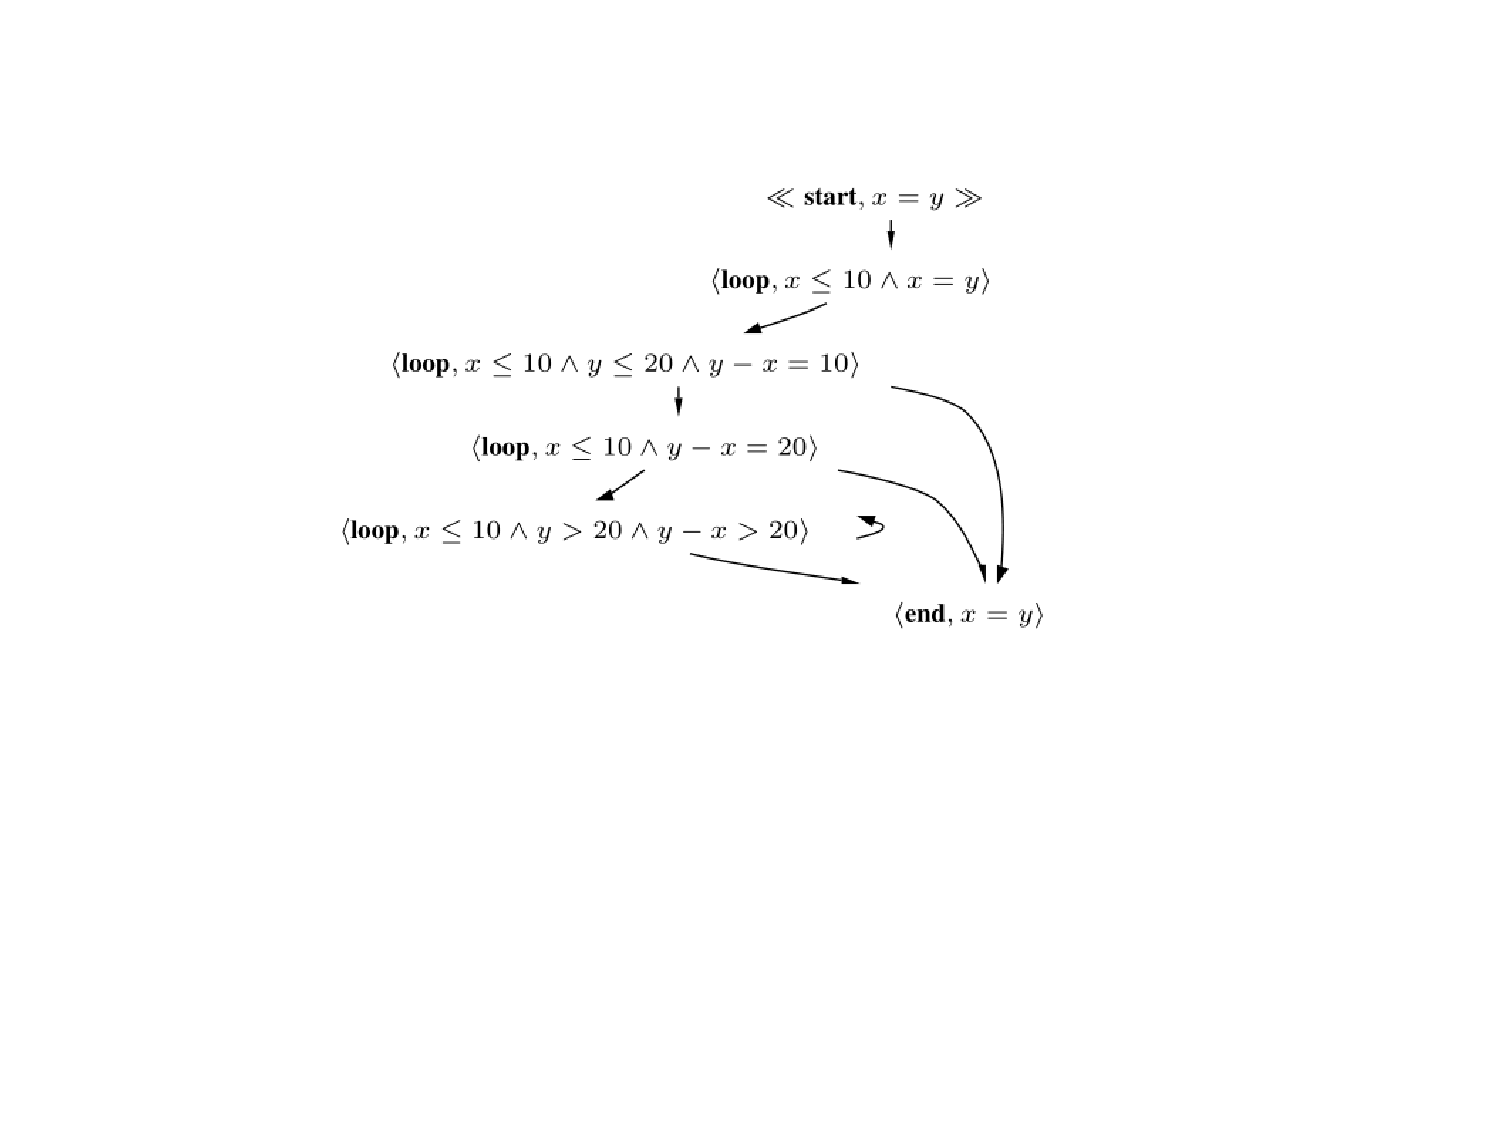
\includegraphics [width=0.7\textwidth] {include/figures/loop_real_zonegraph}%TODO: ezt majd még vektorosítani
%	%		\vspace*{4pt}%
%	\caption{Finite zone graph}
%	\label{fig:looprealgraph}
%\end{figure}
%
%Using normalization the zone graph is finite, but unreachable states may appear in it. If the automaton doesn't have any guard or invarint of the form $c_1 - c_2 < n$, the reachability of the location in question will be answered correctly. Otherwise, the algorithm may terminate with a false positive result.
%
%\begin{example}
%	To demonstrate the incorrectness of the algorithm, consider again the automaton in Figure \ref{fig:splitex}. Recall that the reachabble states of the automaton (by our calculations) were $\langle S0,x=y=z \rangle$, $\langle S1,z \leq x=y \rangle$ and $\langle S2,z \leq y \leq z \leq y \wedge x-y > 2\rangle$ -- $S3$ is unreachable. Applying normalization leaves the states $\langle S0,x=y=z \rangle$ and $\langle S1,z \leq x=y \rangle$ unchanged, but the normalizing the reachable state in $S2$ results in $\langle S2,z \leq y \leq z \leq y \wedge x-y > 1\rangle$, where the guard can be satisfied, thus making $S3$ reachable.
%\end{example}
%
%The operation \emph{split} \cite{bengtsson2004timed} is introduced to assure correctness. Instead of
%normalizing the complete zone, it is first split along the difference constraints,
%then each subzone is normalized, and finally the initially satisfied constraints are reapplied to each normalized subzone. The result is a set of zones (not just one zone like before), which means multiple new nodes have to be introduced to the zone graph (all with edges representing the same transition from the original node).
%
%\begin{example}
%To demonstrate the effects of split, let us construct the zone graph of the automaton of Figure \ref{fig:splitex}. The original node remains  $\langle S0,x=y=z \rangle$, but the next node is first split along the difference constraint $x-z<1$. Instead of the node $\langle S1,z \leq x=y \rangle$, this time there are two nodes: $\langle S1, x=y \wedge x-z<1 \rangle$ and $\langle S1, x=y \wedge x-z \geq 1 \rangle$.
%
%From  $\langle S1, x=y \wedge x-z<1 \rangle$,  $\langle S2,x-z \leq 1 \wedge z-y \leq 1\rangle$ is reachable, where the transition to location $S3$ is not enabled because of the guard $x-z < 1$.
%
%From $\langle S1, x=y \wedge x-z \geq 1 \rangle$ the resulting zone after firing the transition is split along the constraint $z-y<1$, resulting in nodes $\langle S2, x-z \geq 1 \wedge z-y < 1\rangle$, and $\langle S2, x-z \geq 1 \wedge z-y \geq 1\rangle$. The transition to $S3$ is not enabled in either nodes. 
%\end{example}
%
%Applying split results in a zone graph, that is a correct and finite representation of the state space \cite{bengtsson2004timed}.
%
%%\subsection{Implementation}
%
%\todo{Műveletekről, komplexitásról beszélni!!!}
%
%%\emph{Example:}
%%Fischer's protocol assures mutual exclusion by bounding the execution
%%times of the instructions. It can be applied to a number of processes accessing a
%%shared variable. Fig. \ref{fig:fischer}  shows the operation of a process.
%%The location \emph{critical} indicates that the process is in the critical
%%section. The value of the shared variable $id$ ranges between 0 and $n$,
%%where $n$ denotes the number of processes. The model also contains a 
%%clock variable $x_i$ for each process where $i \in \{1 \ldots n\}$ denotes the
%%identifier of the process. The constant $k$ is a parameter of the automaton.
%
%%\begin{figure}
%%	\centering
%%	\begin{minipage}[c] {0.575\linewidth}%
%%		\vspace*{1pt}%
%%		\includegraphics [width=\textwidth]{fischer_vertical}%
%%		\caption{Fischer's protocol}
%%		\label{fig:fischer}
%%	\end{minipage}%
%%	%
%%	\begin{minipage}[c] {0.425\linewidth}%
%%		\includegraphics [width=\textwidth] {fischer_product_1}%
%%		\vspace*{4pt}%
%%		\caption{Timed automaton}
%%		\label{fig:fischer_product}
%%	\end{minipage}
%%\end{figure}  
%
%%\todo{figure}
%
%%The mutual exclusion property would suggest that at any given time
%%at most one of the processes is in the \emph{critical} location. In order to
%%check the given property we must construct a timed automaton that models the
%%operation of a given number of processes.
%
%%As our definition of timed automaton only allows clock variables in the system,
%%everything else must be encoded in the location.
%%  First, to represent the
%% location of all processes simultaneously, we construct a product automaton
%% containing one location for each of the $4^n$ -- not necessarily reachable --
%% possible combinations. 
%% %For example, the initial location will be \{sleeping, sleeping, \ldots \} with
%% % an outgoing edge to each location containing a combination of $n-1$ sleeping
%% % plus one request label and the corresponding invariant. 
%% The $id$ variable can
%% be encoded in the locations the exact same way.
%% The edges, invariants, etc. should be created approriately.
%% Each location of the result automaton will be denoted by a combination of
%% the four original locations and a number representing $id$'s value. 
%%To
%%demonstrate, Fig.
%%\ref{fig:fischer_product} shows the reachable locations of the product automaton
%%of Fischer's protocol where $n=1$. The names of the locations refer to the original locations of the process, the number denotes the value of the variable $id$.
%
%
%\section{CEGAR}
%
%\begin{figure} [b]
%	\centering
%	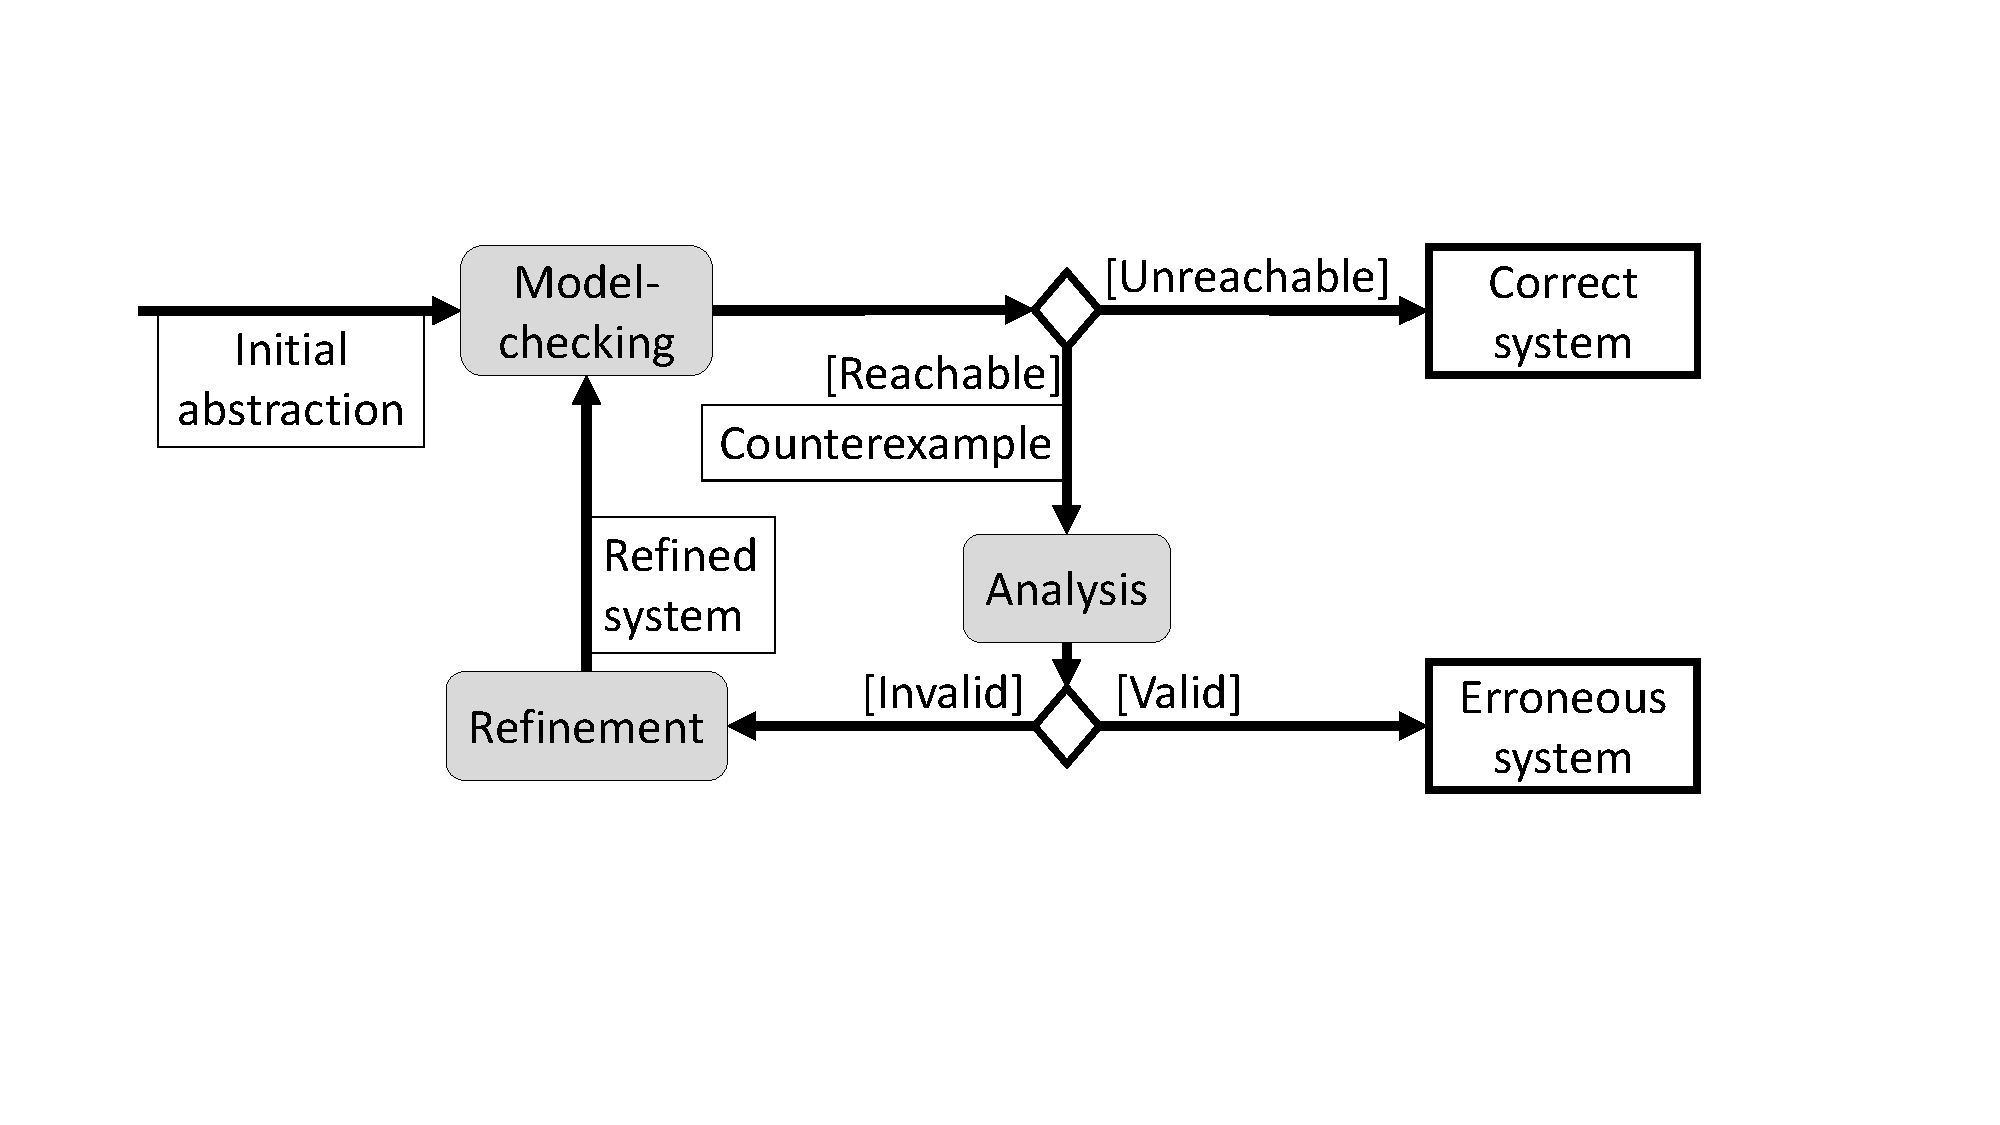
\includegraphics [width=0.7\textwidth] {include/figures/cegar_flow_black}
%	\caption{Counterexample-guided abstraction refinement}
%	\label{fig:cegar}
%\end{figure}
%
%The CEGAR approach introduced in \cite{clarke2003counterexample} makes
%abstraction refinement a key part of model checking. The idea is illustrated on
%Figure \ref{fig:cegar}.
%
%First, an abstract system is constructed. The key idea behind abstraction is
%that the state space of the abstract system overapproximates that of the original
%one. 
%Model checking is performed on this abstract model. If the target state is
%unreachable in the abstract model, it is unreachable in the original model
%as well. Otherwise the model checker produces a counterexample -- a run where the
%system reaches the target state. In our case the counterexample is a sequence of
%transitions -- i.e., a trace. Overapproximation brings such behaviors to the system that are not feasible in the original one. Because of this, the counterexample may not be a valid trace in the real system, so it has to be investigated.
%If it turns
%out to be a feasible counterexample, the target state is reachable. Otherwise
%the abstract system has to be refined. The goal of the refinement is to modify the abstract
%system so that it remains an abstraction of the original one, but the spurious
%counterexample is eliminated.  Model checking is performed on the
%refined system, and the CEGAR loop starts over. 
%
%The algorithm terminates when no more
%counterexamples are found or when a feasible trace is
%given leading to the erroneous state.
%
